\documentclass[11pt]{article}

% Change "review" to "final" to generate the final (sometimes called camera-ready) version.
% Change to "preprint" to generate a non-anonymous version with page numbers.
\usepackage[review]{acl}

% Standard package includes
\usepackage{times}
\usepackage{latexsym}
\usepackage{amsmath}
\usepackage{amssymb}
\usepackage{booktabs} 
% For proper rendering and hyphenation of words containing Latin characters (including in bib files)
\usepackage[T1]{fontenc}
% For Vietnamese characters
% \usepackage[T5]{fontenc}
% See https://www.latex-project.org/help/documentation/encguide.pdf for other character sets

% This assumes your files are encoded as UTF8
\usepackage[utf8]{inputenc}

% This is not strictly necessary, and may be commented out,
% but it will improve the layout of the manuscript,
% and will typically save some space.
\usepackage{microtype}

% This is also not strictly necessary, and may be commented out.
% However, it will improve the aesthetics of text in
% the typewriter font.
\usepackage{inconsolata}

%Including images in your LaTeX document requires adding
%additional package(s)
\usepackage{graphicx}

% If the title and author information does not fit in the area allocated, uncomment the following
%
%\setlength\titlebox{<dim>}
%
% and set <dim> to something 5cm or larger.

\title{Robust Retrieval-Augmented Generation via Textual-Gradient-Guided Adversarial Context Synthesis}

% Author information can be set in various styles:
% For several authors from the same institution:
% \author{Author 1 \and ... \and Author n \\
%         Address line \\ ... \\ Address line}
% if the names do not fit well on one line use
%         Author 1 \\ {\bf Author 2} \\ ... \\ {\bf Author n} \\
% For authors from different institutions:
% \author{Author 1 \\ Address line \\  ... \\ Address line
%         \And  ... \And
%         Author n \\ Address line \\ ... \\ Address line}
% To start a separate ``row'' of authors use \AND, as in
% \author{Author 1 \\ Address line \\  ... \\ Address line
%         \AND
%         Author 2 \\ Address line \\ ... \\ Address line \And
%         Author 3 \\ Address line \\ ... \\ Address line}

\author{First Author \\
  Affiliation / Address line 1 \\
  Affiliation / Address line 2 \\
  Affiliation / Address line 3 \\
  \texttt{email@domain} \\\And
  Second Author \\
  Affiliation / Address line 1 \\
  Affiliation / Address line 2 \\
  Affiliation / Address line 3 \\
  \texttt{email@domain} \\}

%\author{
%  \textbf{First Author\textsuperscript{1}},
%  \textbf{Second Author\textsuperscript{1,2}},
%  \textbf{Third T. Author\textsuperscript{1}},
%  \textbf{Fourth Author\textsuperscript{1}},
%\\
%  \textbf{Fifth Author\textsuperscript{1,2}},
%  \textbf{Sixth Author\textsuperscript{1}},
%  \textbf{Seventh Author\textsuperscript{1}},
%  \textbf{Eighth Author \textsuperscript{1,2,3,4}},
%\\
%  \textbf{Ninth Author\textsuperscript{1}},
%  \textbf{Tenth Author\textsuperscript{1}},
%  \textbf{Eleventh E. Author\textsuperscript{1,2,3,4,5}},
%  \textbf{Twelfth Author\textsuperscript{1}},
%\\
%  \textbf{Thirteenth Author\textsuperscript{3}},
%  \textbf{Fourteenth F. Author\textsuperscript{2,4}},
%  \textbf{Fifteenth Author\textsuperscript{1}},
%  \textbf{Sixteenth Author\textsuperscript{1}},
%\\
%  \textbf{Seventeenth S. Author\textsuperscript{4,5}},
%  \textbf{Eighteenth Author\textsuperscript{3,4}},
%  \textbf{Nineteenth N. Author\textsuperscript{2,5}},
%  \textbf{Twentieth Author\textsuperscript{1}}
%\\
%\\
%  \textsuperscript{1}Affiliation 1,
%  \textsuperscript{2}Affiliation 2,
%  \textsuperscript{3}Affiliation 3,
%  \textsuperscript{4}Affiliation 4,
%  \textsuperscript{5}Affiliation 5
%\\
%  \small{
%    \textbf{Correspondence:} \href{mailto:email@domain}{email@domain}
%  }
%}

\begin{document}
\maketitle
\begin{abstract}
Retrieval-Augmented Generation (RAG) systems often fail when retrieved contexts contain scattered evidence, distracting information, or severe noise, while existing offline robustness training methods struggle to capture diverse and query-specific retrieval failures in real-world scenarios. To address this limitation, we propose TAGS (Textual-Gradient-Guided Adversarial Context Synthesis), a framework for improving the robustness of Retrieval-Augmented Language Models (RALMs) through dynamic adversarial context synthesis. TAGS generates factually correct yet highly challenging adversarial contexts that preserve answer-supporting evidence while increasing the difficulty for RALMs to exploit such evidence. Through an iterative generation--evaluation--feedback process, TAGS converts model feedback into textual gradients to guide adversarial context optimization without relying on predefined noise construction rules. The optimized adversarial contexts are then used for robust fine-tuning, enabling RALMs to better handle noisy and difficult retrieval scenarios. 
Extensive experiments on multiple open-domain question answering benchmarks demonstrate that TAGS substantially improves the robustness and accuracy of RALMs under varying retrieval noise levels and out-of-domain settings. Code is available at \url{https://anonymous.4open.science/r/TTT_tags}.
\end{abstract}



\section{Introduction}

Large language models (LLMs) have achieved remarkable success in natural language understanding and generation tasks \cite{Brown2020Language,Ali2023Performance,achiam2023gpt}. 
However, in knowledge-intensive scenarios, LLMs still suffer from several limitations, including hallucination, outdated knowledge, and insufficient domain coverage \cite{ji2023survey,zhang2023language}. 
\begin{figure}[htbp]
  \centering
  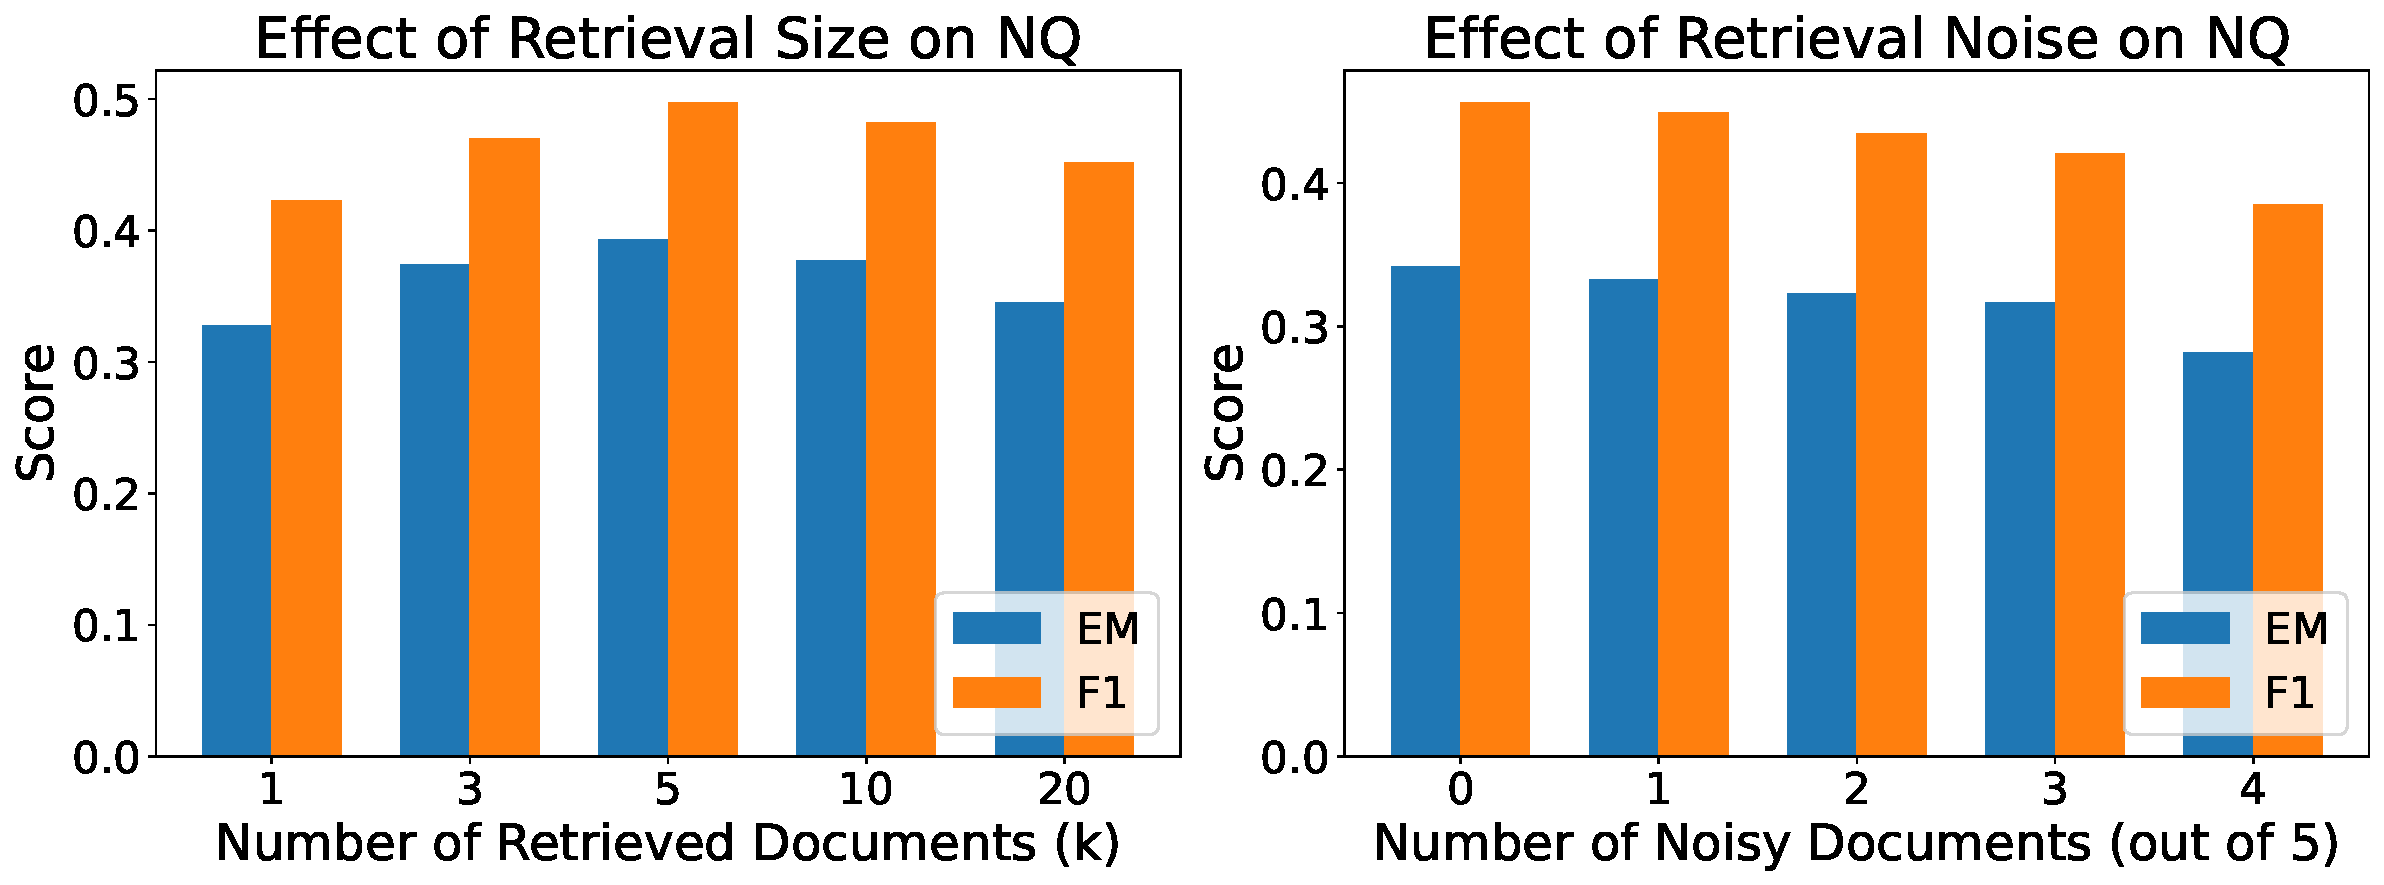
\includegraphics[width=\linewidth]{1.pdf}
  \caption{Sensitivity analysis on Natural Questions. Left: performance as retrieval depth $k$ increases. Right: performance as answer-supporting documents are progressively replaced by low-ranked distractors.}
  \label{fig:retrieval_sensitivity}
\end{figure}
Retrieval-Augmented Generation (RAG) mitigates these issues by incorporating external documents as contextual knowledge and has become a widely adopted framework for open-domain question answering and knowledge-intensive applications \cite{lewis2020retrieval,guu2020retrieval,fan2024survey}.



Despite its effectiveness, the performance of RAG systems is highly dependent on the quality and usability of retrieved contexts. 
Previous studies have shown that retrieval relevance alone is insufficient to guarantee reliable generation: even when retrieved documents contain the correct answer, models may still fail to extract useful evidence when the context contains distracting information, noisy documents, or complex semantic interference \cite{shi2023large,yoran2023making}. 
As retrieval noise increases, RAG models often experience significant performance degradation, indicating that retrieval defects affect not only relevance but also the stability of model reasoning \cite{cuconasu2024power,amiraz-etal-2025-distracting}.


To improve the robustness of RAG systems, existing studies mainly focus on offline training strategies, including noise-aware fine-tuning, adversarial training, and context-aware reasoning mechanisms \cite{RbFT,RAAT,ATM,CoN}. 
However, these approaches usually rely on manually designed perturbations or predefined noise distributions, which limits their ability to cover the diverse and evolving failure patterns encountered in real-world retrieval systems. 
In particular, retrieval failures are often query-specific and context-dependent, making it difficult for a fixed training distribution to expose all potential weaknesses of RAG models.


This motivates a fundamental question:
\textit{Can we automatically discover context-specific weaknesses of RAG models and synthesize targeted training data according to model feedback?}


Recent studies suggest that model behaviors and generation feedback provide valuable signals for improving text generation and optimization \cite{textgrad,tpo}. 
Instead of exhaustively enumerating possible retrieval failures during data construction, leveraging feedback from model responses under challenging contexts provides a promising direction for constructing more effective robustness training data.


In this work, we propose TAGS (Textual-Gradient-Guided Adversarial Context Synthesis), a framework for improving the robustness of Retrieval-Augmented Language Models (RALMs). 
The key idea of TAGS is to dynamically synthesize challenging adversarial contexts based on model feedback and transform the discovered weaknesses into effective robustness supervision.


Specifically, TAGS introduces a frozen attacker model to generate candidate adversarial contexts conditioned on the query and the original retrieval context. 
These adversarial contexts preserve answer-supporting evidence while making such evidence more difficult for RALMs to reliably utilize. 
Through an iterative \textbf{generation--evaluation--feedback process}, TAGS evaluates candidate contexts according to the target RALM's behaviors, converts preference signals into natural-language \textbf{textual gradients}, and uses them to guide subsequent adversarial context optimization.


After iterative optimization, the generated adversarial contexts are filtered and incorporated into robust fine-tuning, enabling RALMs to better handle noisy and difficult retrieval scenarios. 
Unlike existing robustness methods that depend on predefined noise construction rules, TAGS dynamically identifies and synthesizes query-specific challenging contexts according to model feedback, providing more effective supervision for improving RAG robustness.


In this work, \emph{adversarial contexts} refer to semantically modified retrieval contexts that preserve answer-supporting evidence while increasing the difficulty for the target RALM to exploit such evidence. 
They are designed to simulate challenging retrieval conditions, such as evidence dilution, information reordering, and distracting content, rather than malicious attacks such as corpus poisoning, malicious evidence injection, or targeted attacks on retrieval systems.


The main contributions of this work are summarized as follows:

\begin{itemize}
    \item We propose TAGS (Textual-Gradient-Guided Adversarial Context Synthesis), a framework for RAG robustness enhancement that dynamically constructs query-specific adversarial contexts through an iterative generation--evaluation--feedback process.

    \item We introduce textual gradients as optimization signals for adversarial context synthesis, enabling the generation of factually correct yet highly challenging contexts without relying on predefined noise construction rules.

    \item Extensive experiments on multiple open-domain question answering benchmarks demonstrate that TAGS substantially improves the robustness and accuracy of RALMs under varying retrieval noise levels and out-of-domain settings.
\end{itemize}

\section{Related Work}

\subsection{Robustness of Retrieval-Augmented Generation}

Irrelevant or difficult-to-use retrieval contexts can substantially degrade answer generation, and semantically related but misleading contexts can be particularly harmful \cite{shi2023large,cuconasu2024power,amiraz-etal-2025-distracting}. 
RetRobust improves robustness by training with both relevant and irrelevant contexts to mitigate the impact of distracting retrieval results \cite{yoran2023making}. 
Other approaches leverage note-based relevance reasoning \cite{CoN} or instruction and rationale tuning \cite{instructrag}. 
RbFT enhances robustness through defect-aware training with sampled or synthetically corrupted contexts \cite{RbFT}. 
RAAT adopts adaptive adversarial training with noise recognition \cite{RAAT}, while ATM improves robustness through iterative optimization between an attacker model and an answer generator \cite{ATM}. 
Different from these approaches that mainly rely on predefined perturbations or adversarial training objectives, TAGS dynamically synthesizes query-specific adversarial contexts through textual gradients and uses the synthesized contexts for robust fine-tuning of the target RALM.


\subsection{Textual Feedback and Adversarial Context Synthesis}

Recent studies demonstrate that natural-language feedback can serve as an effective optimization signal for text generation and refinement. 
TextGrad introduces textual gradients to optimize text-valued variables through language-model-generated feedback \cite{textgrad}. 
Test-Time Preference Optimization further explores iterative textual feedback for improving model responses without conventional parameter updates \cite{tpo}.

Different from previous methods that optimize generated responses or model behaviors, TAGS applies textual feedback to a new optimization target: adversarial contexts for robustness enhancement. 
Specifically, the target RALM's responses provide evaluation signals for ranking candidate contexts, while contrastive feedback between candidates guides subsequent adversarial context optimization. 
Parameter learning occurs only after context synthesis, through supervised fine-tuning on the selected adversarial contexts.
\section{Method}

We propose TAGS (Textual-Gradient-Guided Adversarial Context Synthesis), a framework for improving the robustness of Retrieval-Augmented Language Models (RALMs). 
The key idea of TAGS is to dynamically synthesize query-specific adversarial contexts based on model feedback and transform the discovered weaknesses into effective robustness supervision.

TAGS consists of two stages:
(1) adversarial context synthesis, where a frozen auxiliary attacker model generates and optimizes challenging retrieval contexts through textual gradients;
(2) robust fine-tuning, where the target RALM is optimized using the synthesized contexts.

During adversarial context synthesis, all model parameters remain frozen. 
Parameter updates are only performed in the subsequent supervised fine-tuning stage.


\subsection{Problem Definition}

Given a query $q$, a retrieved context $\mathcal{R}_{K}(q)$, and a reference answer $y^*$, TAGS aims to construct adversarial contexts that improve the robustness of RALMs under noisy and difficult retrieval scenarios.

An adversarial context $d$ is defined as a semantically modified version of the original retrieval context $\mathcal{R}_{K}(q)$ that preserves answer-supporting evidence while increasing the difficulty for the target RALM to effectively utilize such evidence.

Unlike malicious retrieval attacks, TAGS focuses on realistic retrieval failures, including evidence dilution, information reordering, and distracting contexts. 
Therefore, adversarial contexts are designed to challenge evidence utilization rather than remove or inject unsupported knowledge.


\subsection{Textual-Gradient-Guided Adversarial Context Synthesis}

Given a training instance $(q,\mathcal{R}_{K}(q),y^*)$, TAGS first employs a frozen auxiliary attacker model $A_{\phi}$ to generate candidate adversarial contexts.

\paragraph{Initial context generation.}

The attacker receives the query, reference answer, and the complete retrieved context, and generates an initial candidate set:

\begin{equation}
\mathcal{D}^{(0)}_q
=
\{d^{(0)}_1,\ldots,d^{(0)}_n\},
\end{equation}

where

\begin{equation}
d^{(0)}_i
\sim
A_{\phi}(\cdot|q,\mathcal{R}_{K}(q),y^*).
\end{equation}

Each candidate $d_i$ contains a semantic rewrite of the complete top-$K$ retrieved context. 
The attacker is instructed to preserve factual correctness and answer-supporting evidence while introducing challenges such as paraphrasing, information reordering, and evidence dilution.


\paragraph{Context evaluation and reward modeling.}

For each candidate adversarial context $d_i^{(t)}$, the frozen target RALM generates:

\begin{equation}
y_i^{(t)}
=
f_{\theta}(q,d_i^{(t)}).
\end{equation}

The original retrieval context $\mathcal{R}_{K}(q)$ is not provided together with $d_i^{(t)}$, preventing the target RALM from bypassing the synthesized context by directly accessing the original evidence.

We evaluate each candidate using a weighted reward:

\begin{equation}
\begin{aligned}
r(d_i,y_i,y^*)=
&\alpha r_{\mathrm{ans}}(y_i,y^*)\\
&+\beta r_{\mathrm{unc}}(y_i;q,d_i)\\
&+\gamma r_{\mathrm{evid}}(q,d_i,y^*).
\end{aligned}
\end{equation}
For simplicity, we denote the reward of a candidate context $d_i$ as $r(d_i)$ hereafter.
\begin{figure*}[t]
  \centering
  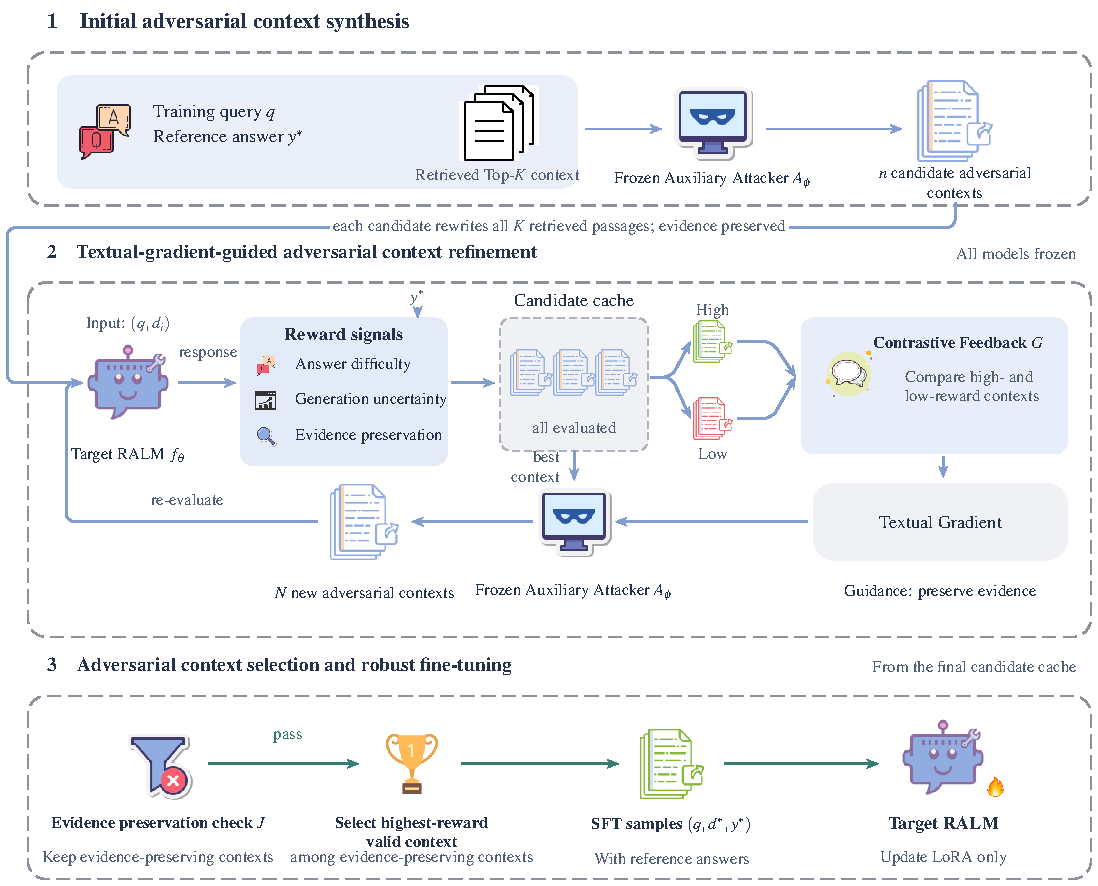
\includegraphics[width=\linewidth]{latex/v3.pdf}
  \caption{Overview of TAGS.
TAGS first synthesizes query-specific adversarial contexts through an iterative generation--evaluation--feedback process.
A frozen auxiliary attacker model generates candidate contexts, and textual gradients derived from contrastive feedback guide context optimization.
The selected adversarial contexts are then used for LoRA-based robust fine-tuning of the target RALM.
During inference, only the retriever and the fine-tuned RALM are required.}
  \label{fig:framework}
\end{figure*}
The three components are defined as:

\begin{equation}
r_{\mathrm{ans}}(y_i,y^*)
=
-\left(
EM(y_i,y^*)+F1(y_i,y^*)
\right),
\end{equation}

which encourages contexts that cause the target RALM to deviate from the reference answer.


\begin{equation}
r_{\mathrm{unc}}(y_i;q,d_i)
=
\log
(1+PPL_{\theta}(y_i|q,d_i)),
\end{equation}

which measures generation uncertainty under the candidate context.


\begin{equation}
r_{\mathrm{evid}}(q,d_i,y^*)
=
\mathbb{I}
[J(q,d_i,y^*)=\textsc{Yes}],
\end{equation}

which ensures that the candidate context still contains sufficient evidence supporting the reference answer.

The final reward balances three objectives:
inducing generation difficulty, increasing model uncertainty, and preserving answer-supporting evidence.
We use fixed weights across datasets:
$\alpha=1.0$, $\beta=0.5$, and $\gamma=2.0$.


\paragraph{Contrastive textual gradient optimization.}

At iteration $t$, TAGS maintains a candidate cache $\mathcal{C}^{(t)}_q$ containing previously evaluated contexts.

The highest- and lowest-reward contexts are selected:

\begin{equation}
d_t^+
=
\arg\max_{d\in\mathcal{C}^{(t)}_q}r(d),
\end{equation}


\begin{equation}
d_t^-
=
\arg\min_{d\in\mathcal{C}^{(t)}_q}r(d).
\end{equation}


A frozen feedback model compares the two contexts and generates a textual gradient:

\begin{equation}
g_{\mathrm{text}}^{(t)}
=
G(q,\mathcal{R}_{K}(q),d_t^+,d_t^-),
\end{equation}

where the textual gradient describes why $d_t^+$ is more challenging than $d_t^-$ while maintaining factual correctness. Unlike numerical gradients that update model parameters, textual gradients provide natural-language optimization directions for refining adversarial contexts.

Conditioned on the current best context and textual gradient, the attacker generates new candidates:

\begin{equation}
\mathcal{D}^{(t+1)}_q
=
\{d_j^{(t+1)}\}_{j=1}^{N}
\sim
A_{\phi}
(\cdot|d_t^+,g_{\mathrm{text}}^{(t)}).
\end{equation}

This iterative generation--evaluation--feedback process continues until the synthesized contexts converge.


\subsection{Robust Fine-tuning}

After adversarial context synthesis, TAGS selects the highest-quality context:

\begin{equation}
d^*
=
\arg\max_{d\in\mathcal{V}_q}r(d),
\end{equation}

where $\mathcal{V}_q$ denotes candidates passing the evidence-preservation check.

The selected triples:

\begin{equation}
(q,d^*,y^*)
\end{equation}

form the supervised fine-tuning dataset.

We optimize the target RALM using LoRA with the standard supervised objective:

\begin{equation}
\mathcal{L}_{SFT}
=
-
\mathbb{E}_{(q,d^*,y^*)}
[
\log p_{\theta}(y^*|q,d^*)
].
\end{equation}

During this stage, only the target RALM parameters are updated.
The auxiliary attacker model and feedback model remain frozen.


\subsection{Train--Test Separation}

All adversarial context synthesis, reward computation, textual gradient generation, and LoRA updates are performed exclusively on training instances.

Held-out evaluation queries are never involved in context synthesis or model optimization.

During inference, TAGS only requires the retriever and the fine-tuned target RALM.
No attacker model, textual gradient generation, reference answer, or additional parameter update is involved.

% \section{Method}
% \subsection{Problem Definition}

% Given a query $q$, retrieved context $\mathcal{R}(q)$, and reference answer $y^*$, TAGS aims to construct adversarial contexts that improve the robustness of Retrieval-Augmented Language Models (RALMs).

% Here, adversarial contexts refer to semantically modified retrieval contexts that preserve answer-supporting evidence while increasing the difficulty for the target RALM to exploit such evidence.

% Different from malicious retrieval attacks, such as corpus poisoning or targeted retrieval manipulation, TAGS focuses on simulating realistic retrieval failures, including evidence dilution, information reordering, and distracting contexts.
% \begin{figure*}[t]
%   \centering
%   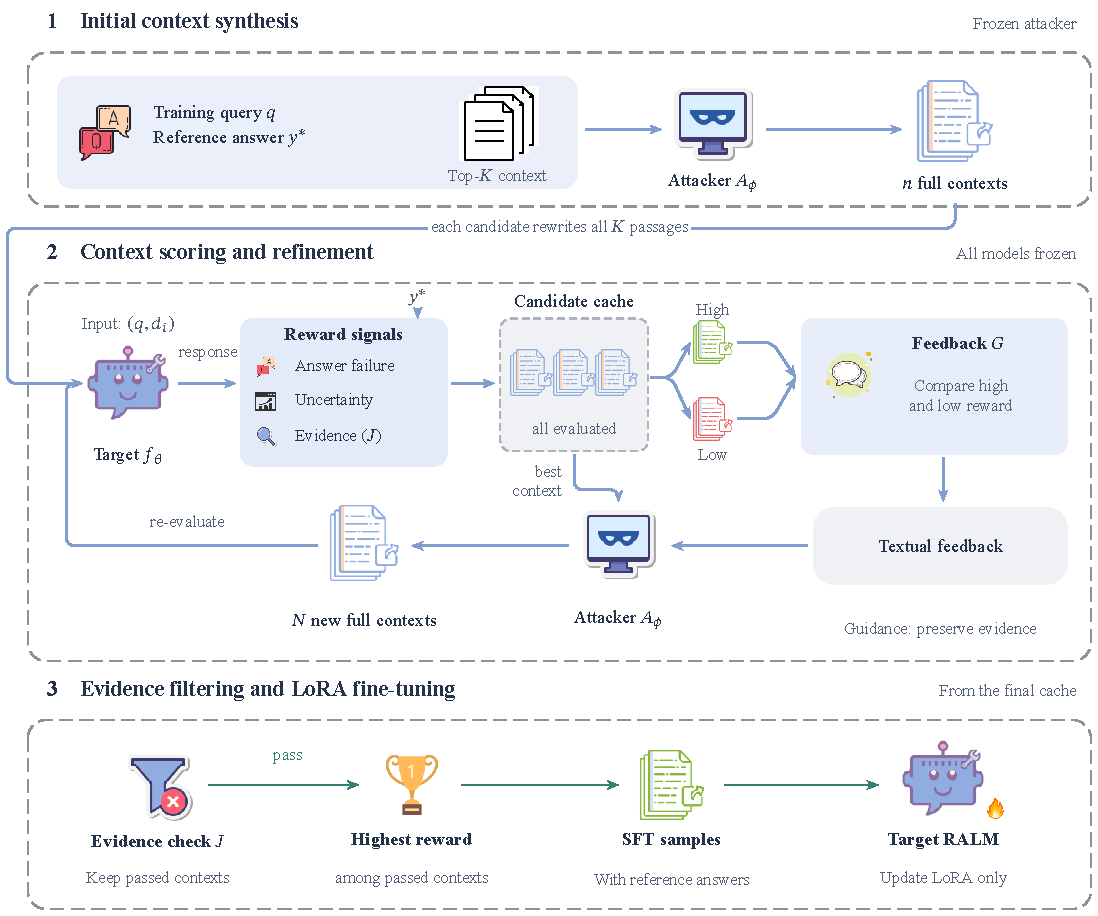
\includegraphics[width=\linewidth]{latex/framework_优化.pdf}
%   \caption{Overview of offline synthesis, supervised fine-tuning, and inference. Stage I scores complete top-$K$ context rewrites with a frozen target RALM and uses contrastive textual feedback to guide a frozen attacker. Only candidates passing the evidence check are eligible for final training-data selection. Stage II fine-tunes the target with LoRA. Prediction uses only the retriever and fine-tuned target model.}
%   \label{fig:framework}
% \end{figure*}

% Figure~\ref{fig:framework} summarizes the pipeline. A labeled training instance is $(q,\mathcal{R}_{K}(q),y^*)$, where $q$ is a query, $\mathcal{R}_{K}(q)=[p_1,\ldots,p_K]$ is the complete top-$K$ retrieved context, and $y^*$ is the reference answer. Stage~I uses an attacker $A_{\phi}$ and a target RALM $f_{\theta}$ with fixed parameters. Stage~II trains LoRA adapters for the target RALM on the selected contexts.

% \subsection{Stage I: Textual-Gradient-Guided Context Synthesis}

% \paragraph{Initial candidates.}
% The attacker receives the query, reference answer, and a serialization of all $K$ retrieved passages. It generates an initial pool of $n$ evidence-preserving rewrites:
% \begin{equation}
% \begin{aligned}
% \mathcal{D}^{(0)}_q&=\{d^{(0)}_1,\ldots,d^{(0)}_n\},\\
% d^{(0)}_i&\sim A_{\phi}(\cdot\mid q,\mathcal{R}_{K}(q),y^*).
% \end{aligned}
% \end{equation}
% Each $d_i$ contains a rewrite of all $K$ retrieved passages and is evaluated as one complete context. The attacker is instructed to preserve facts and answer-supporting evidence while paraphrasing, reordering, or redistributing information across those passages. These instructions define the intended perturbation; the final evidence check determines which candidates are eligible for training.

% \paragraph{Target-model response and reward.}
% For every candidate $d_i^{(t)}$, the frozen target RALM generates
% \begin{equation}
% y_i^{(t)} = f_{\theta}(q,d_i^{(t)}).
% \end{equation}
% The original context $\mathcal{R}_{K}(q)$ is not supplied alongside $d_i^{(t)}$; otherwise, the target could bypass the rewrite and copy explicit evidence from the original passages. We score a candidate using its generated response and the reference answer:
% \begin{equation}
% \begin{aligned}
% r(q,d_i,y_i,y^*) ={}& \alpha\,r_{\mathrm{ans}}(y_i,y^*) \\
% &+ \beta\,r_{\mathrm{conf}}(y_i;q,d_i) \\
% &+ \gamma\,r_{\mathrm{evid}}(q,d_i,y^*).
% \end{aligned}
% \label{eq:reward}
% \end{equation}
% The three terms capture complementary requirements:
% \begin{align}
% r_{\mathrm{ans}}(y_i,y^*)
%   &= -\bigl(\operatorname{EM}(y_i,y^*)+\operatorname{F1}(y_i,y^*)\bigr),\\
% r_{\mathrm{conf}}(y_i;q,d_i)
%   &= \log\bigl(1+\operatorname{PPL}_{\theta}(y_i\mid q,d_i)\bigr),\\
% r_{\mathrm{evid}}(q,d_i,y^*)
%   &= \mathbb{I}\!\left[J(q,d_i,y^*)=\textsc{Yes}\right].
% \end{align}
% The answer term favors target-model failures. The confidence term uses the perplexity of the target's generated response as an uncertainty proxy, rather than a calibrated confidence estimate. The evidence term records whether a frozen judge $J$ finds support for the reference answer in the candidate context. These terms determine candidate ranking; a high total reward alone does not guarantee evidence preservation. Final selection additionally requires the candidate to pass the evidence check. We use fixed weights across datasets: $\alpha=1.0$, $\beta=0.5$, and $\gamma=2.0$, without dataset-specific tuning.

% \paragraph{Contrastive textual feedback.}
% At iteration $t$, the cache $\mathcal{C}^{(t)}_q$ contains the candidates evaluated so far. Each candidate is stored with its target response and reward from Equation~\ref{eq:reward}; $r(d)$ below abbreviates this score for the current query and reference answer. We select
% \begin{equation}
% d^{+}_t=\arg\max_{d\in\mathcal{C}^{(t)}_q}r(d),\qquad
% d^{-}_t=\arg\min_{d\in\mathcal{C}^{(t)}_q}r(d).
% \end{equation}
% Here $d^{+}_t$ and $d^{-}_t$ are the highest- and lowest-reward cached contexts. Their ranking does not by itself establish eligibility for final selection. A frozen feedback model compares the pair and produces a textual gradient
% \begin{equation}
% g^{(t)}_{\mathrm{text}}
% =G(q,\mathcal{R}_{K}(q),d^{+}_t,d^{-}_t),
% \end{equation}
% which explains what makes the stronger candidate more disruptive without proposing factual changes. Conditioned on $d^{+}_t$ and $g^{(t)}_{\mathrm{text}}$, the attacker generates $N$ new candidates:
% \begin{equation}
% \mathcal{D}^{(t+1)}_q
% =\{d^{(t+1)}_j\}_{j=1}^{N}
% \sim A_{\phi}(\cdot\mid d^{+}_t,g^{(t)}_{\mathrm{text}}).
% \end{equation}
% Here $n$ is the initial pool size and $N$ is the number of new candidates per synthesis round. The textual gradient guides a prompt-based update to the context, with no parameter updates. Let $\mathcal{C}_q$ be the final cache of evaluated candidates and let $\mathcal{V}_q$ contain those that pass the final evidence-preservation check. Selection is restricted to this eligible subset: \begin{equation} d^*\in\arg\max_{d\in\mathcal{V}_q} r(d),\qquad \mathcal{V}_q\subseteq\mathcal{C}_q. \label{eq:final_selection}\end{equation} Thus, a candidate that fails the check cannot be selected solely because of a high reward. Appendix~\ref{sec:synthesis_algorithm} summarizes the procedure.

% \subsection{Stage II: Supervised Robust Fine-Tuning}
% The selected triples $(q,d^*,y^*)$ form the offline fine-tuning set $\mathcal{D}_{\mathrm{SFT}}$. We train the target RALM's LoRA adapters with the standard supervised objective
% \begin{equation}
% \mathcal{L}_{\mathrm{SFT}}
% =-\mathbb{E}_{(q,d^*,y^*)\sim\mathcal{D}_{\mathrm{SFT}}}
% \left[\log p_{\theta}(y^*\mid q,d^*)\right].
% \end{equation}
% This objective trains the model to produce the reference answer from the selected difficult context. The attacker and feedback models are not involved in this stage or in deployment.

% \subsection{Train--Test Separation}
% Context synthesis, synthesis rewards, candidate selection, and LoRA updates use only training instances and their reference answers. Held-out queries do not enter either training stage. At prediction time, the fine-tuned RALM receives the query and retrieved context, without a reference answer, attacker calls, or parameter updates. Reference answers are used separately to construct the common context-sufficient evaluation subset and to compute EM and F1, as described in Section~\ref{sec:exp_settings}. These evaluation uses do not feed back into synthesis or training.
\section{Experimental Settings}


\subsection{Tasks, Datasets, and RAG Setup}
\label{sec:exp_settings}

We evaluate TAGS on five open-domain question answering benchmarks: Natural Questions (NQ) \cite{kwiatkowski2019natural}, PopQA \cite{popqa}, HotpotQA \cite{hotpotqa}, 2WikiMultiHopQA \cite{2wqa}, and the DAE difficult-context evaluation set.

DAE is strictly held out from adversarial context synthesis, candidate selection, and model optimization.

All methods use the same retrieve-then-read pipeline implemented with FlashRAG \cite{Flash}, the \texttt{e5-base-v2} dense retriever, and top-$K$ retrieval with $K=5$. We report Exact Match (EM) and token-level F1.

The target RALM is initialized with LLaMA-3.2-3B-Instruct. During adversarial context synthesis, TAGS uses Qwen3-32B as the frozen auxiliary attacker model. The auxiliary model is only used for offline context synthesis and is not involved during inference.

\begin{table}[b]
\centering
\small
\begin{tabular}{lrr}
\toprule
\textbf{Dataset} & \textbf{Test} & \textbf{Retain} \\
\midrule
\text{Natural Questions} (\text{NQ}) & 3,610 & 982 \\
\text{PopQA} & 1,399 & 751 \\
\text{HotpotQA} & 7,404 & 348 \\
\text{2WikiMultiHopQA} & 12,576 & 210 \\
\text{DAE} & 982 & 774 \\
\bottomrule
\end{tabular}
\caption{Statistics of the evaluated datasets after context sufficiency filtering. ``Test'' denotes the original test set size, and ``Retain'' denotes the number of instances retained for evaluation.}
\label{tab:dataset_stats}
\end{table}

\subsection{Retrieval Difficulty Construction and Robustness Evaluation}

To evaluate robustness under challenging retrieval scenarios, we construct retrieval difficulty settings by progressively replacing highly ranked documents with lower-ranked retrieved distractors.
For each query, we retrieve the top-50 documents and keep the number of input documents fixed at five.We gradually replace high-ranked documents with documents from ranks 47--50, producing five difficulty levels.
These distractors are naturally retrieved documents under the same retriever. They remain semantically related to the query but are less likely to contain answer-supporting evidence.
Therefore, this evaluation measures robustness to realistic retrieval difficulty, such as evidence dilution and distracting contexts, rather than synthetic malicious attacks.
\subsection{Retrieval Noise Construction and Robustness Evaluation Settings}
\begin{table}[b]
  \centering
  \caption{Retrieval difficulty settings with progressively increasing distractor ratios.}
  \label{tab:noise_setting}
  \setlength{\tabcolsep}{15pt}
  \renewcommand{\arraystretch}{1.1}
  \begin{tabular}{cl}
  \toprule
  \textbf{Setting} & \textbf{Retrieved Context} \\
  \midrule
  0 & Top1--5 \\
  1 & Top1--4 + Rank50 \\
  2 & Top1--3 + Rank49--50 \\
  3 & Top1--2 + Rank48--50 \\
  4 & Top1 + Rank47--50 \\
  \bottomrule
  \end{tabular}
\end{table}
\label{sec:noise_setting}
For each query, we retrieve the top-50 documents and keep the number of input documents fixed at five. We then progressively replace high-ranked documents with documents from ranks 47--50, producing the five settings in Table~\ref{tab:noise_setting}. These low-ranked documents remain semantically close to the query under the same retriever but are less likely to contain answer-supporting evidence, so they serve as naturally retrieved distractors rather than synthetic malicious content. We apply this controlled evaluation to NQ, PopQA, HotpotQA, and 2WikiMultiHopQA.
\begin{table*}[t]
\caption{Held-out robustness comparison across five QA benchmarks. Best results in each column are shown in bold. $^*$ marks a significant improvement over LLaMA3.2-3B under a two-sided paired $t$-test on per-example scores ($p<0.05$).}
\label{tab:rag_robustness}
\centering
\small
\setlength{\tabcolsep}{5pt}
\renewcommand{\arraystretch}{1.05}
\begin{tabular*}{\textwidth}{@{\extracolsep{\fill}}lcccccccccc}
\toprule
\textbf{Model} 
& \multicolumn{2}{c}{\textbf{NQ}} 
& \multicolumn{2}{c}{\textbf{POPQA}} 
& \multicolumn{2}{c}{\textbf{DAE}} 
& \multicolumn{2}{c}{\textbf{HotpotQA}} 
& \multicolumn{2}{c}{\textbf{2WikiMultiHopQA}} \\
\cmidrule(lr){2-3}\cmidrule(lr){4-5}\cmidrule(lr){6-7}\cmidrule(lr){8-9}\cmidrule(lr){10-11}
& EM & F1 & EM & F1 & EM & F1 & EM & F1 & EM & F1 \\
\midrule
LLaMA3.2-3B  & 0.441 & 0.573 & 0.667 & 0.765 & 0.052 & 0.157 & 0.434 & 0.555 & 0.414 & 0.501 \\
LLaMA3-8B    & 0.426 & 0.566 & 0.642 & 0.772 & 0.169 & 0.315 & 0.402 & 0.549 & 0.290 & 0.438 \\
Qwen3-4B     & 0.241 & 0.417 & 0.601 & 0.715 & 0.071 & 0.232 & 0.402 & 0.549 & 0.286 & 0.457 \\
Qwen3-8B     & 0.333 & 0.496 & 0.587 & 0.732 & 0.097 & 0.205 & 0.483 & 0.612 & 0.470 & 0.563 \\
RbFT         & 0.485 & 0.586 & 0.579 & 0.661 & 0.371 & 0.490 & 0.480 & 0.595 & 0.390 & 0.469 \\
ATM          & 0.470 & 0.598 & 0.419 & 0.486 & 0.264 & 0.389 & 0.250 & 0.336 & 0.176 & 0.242 \\
RAAT         & 0.382 & 0.483 & 0.704 & 0.747 & 0.161 & 0.275 & 0.394 & 0.500 & 0.405 & 0.480 \\
\midrule
\textbf{Ours} 
& \textbf{0.506}$^{*}$ & \textbf{0.625}$^{*}$ 
& \textbf{0.727}$^{*}$ & \textbf{0.804}$\,$ 
& \textbf{0.513}$^{*}$ & \textbf{0.663}$^{*}$ 
& \textbf{0.486}$\,$ & \textbf{0.629}$^{*}$ 
& \textbf{0.524}$\,$ & \textbf{0.619}$^{*}$ \\
\bottomrule
\end{tabular*}
\end{table*}

\subsection{Baselines}

We compare TAGS with two categories of baselines.

First, we include instruction-tuned backbone models, including LLaMA-3.2-3B-Instruct, LLaMA-3-8B, Qwen3-4B, and Qwen3-8B, which measure the robustness of standard RALM pipelines without additional robustness training.

Second, we compare against representative robustness-oriented RAG methods, including RbFT \cite{RbFT}, ATM \cite{ATM}, and RAAT \cite{RAAT}.

All methods share the same retriever, retrieved contexts, answer prompts, decoding settings, evaluation metrics, and context-sufficiency filtering procedure.

For TAGS, the auxiliary attacker model is only used during offline adversarial context synthesis and is not involved in inference.

\section{Results and Analysis}
We organize the analysis around five research questions:
\begin{itemize}
    \item \textbf{RQ1:} How does TAGS compare with existing robustness-oriented RAG methods?
    \item \textbf{RQ2:} How does TAGS perform under increasing retrieval difficulty?
    \item \textbf{RQ3:} Does contrastive selection of adversarial contexts improve synthesis quality?
    \item \textbf{RQ4:} How does the number of synthesis iterations affect TAGS performance?
    \item \textbf{RQ5:} What contribution does textual feedback provide compared with fixed feedback?
\end{itemize}


\begin{figure}[t]
  \centering
  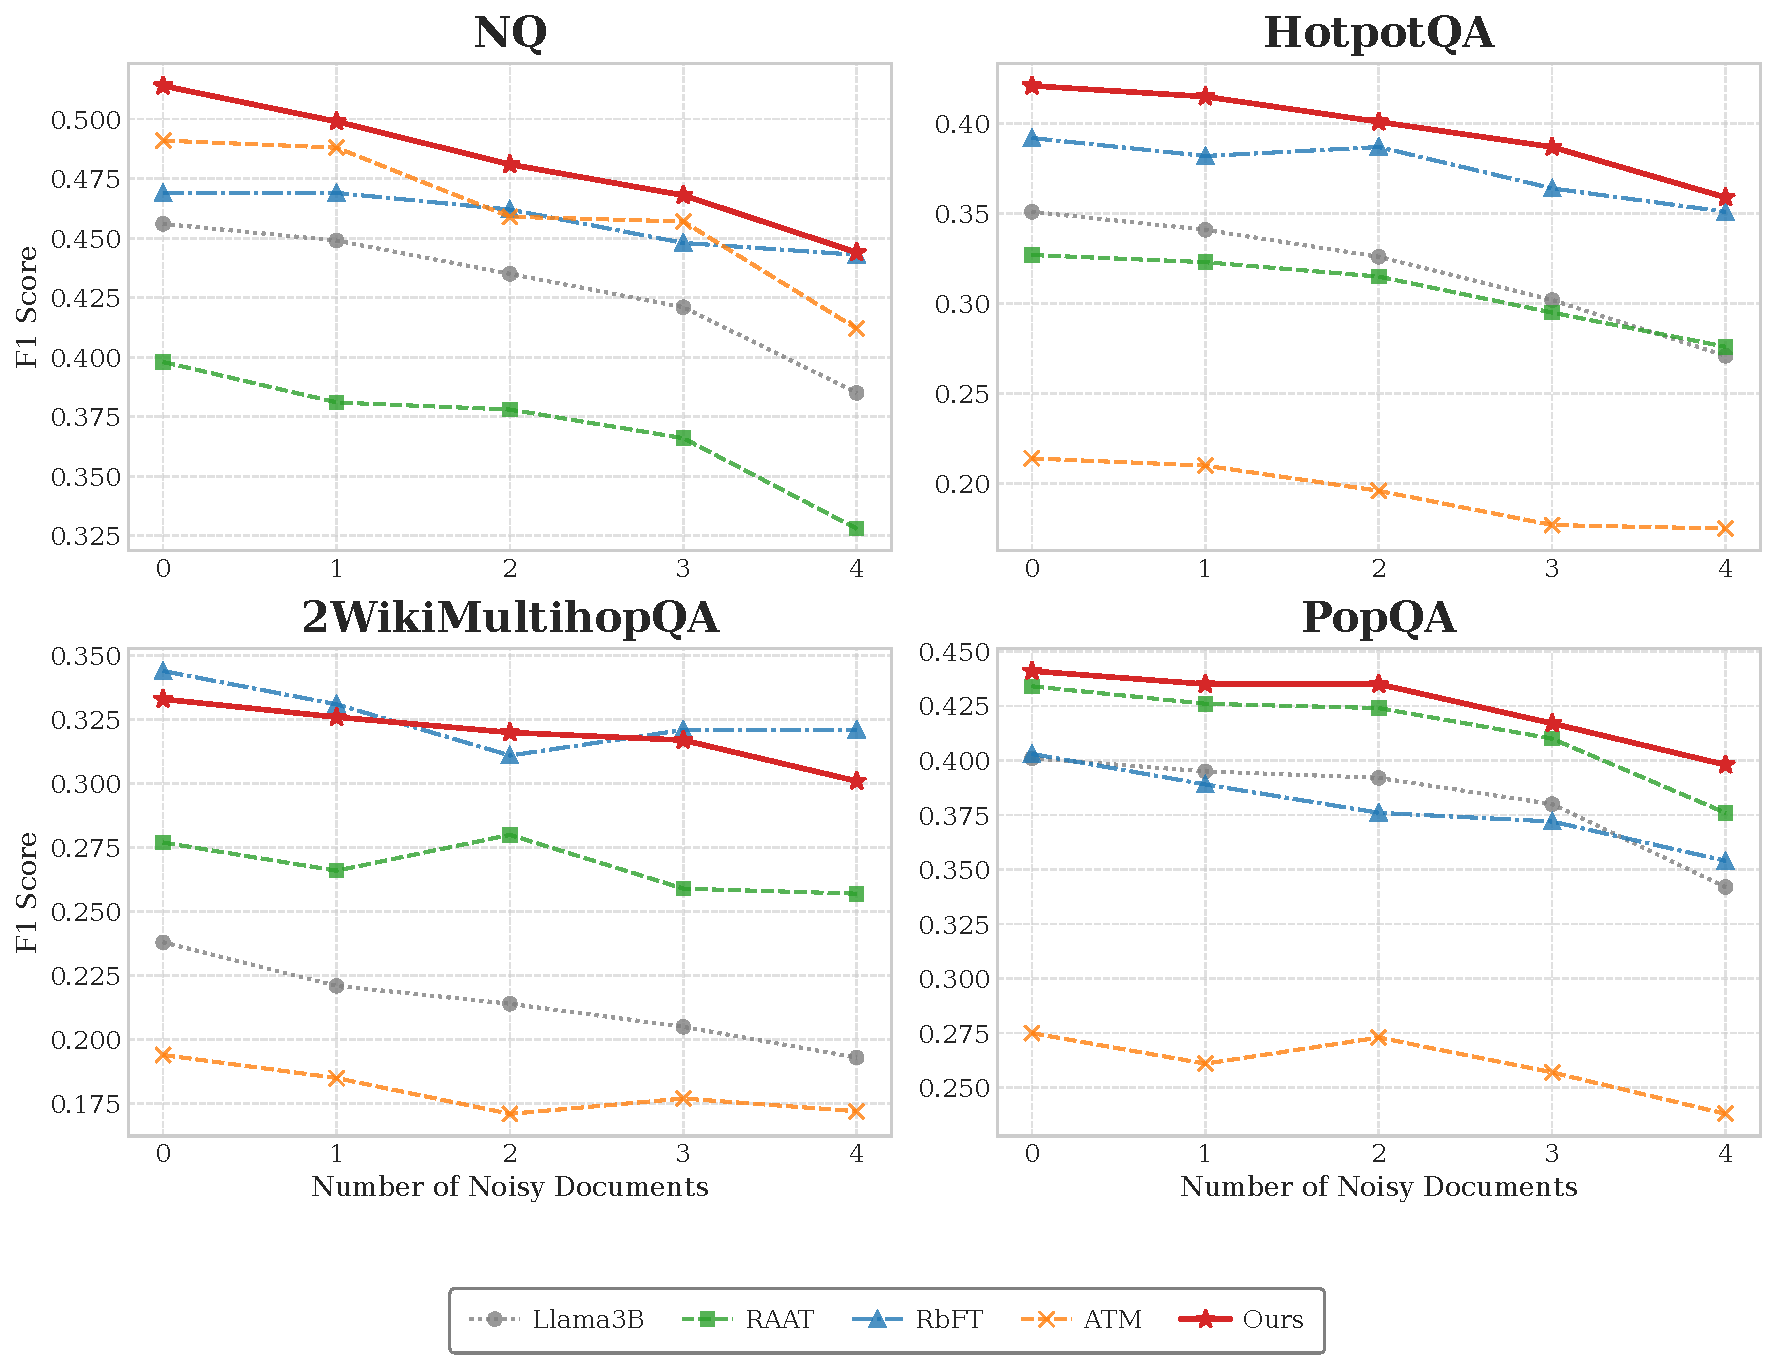
\includegraphics[width=\linewidth]{rag_robustness.pdf}
  \caption{F1 as the number of low-ranked distractors increases on NQ, HotpotQA, 2WikiMultiHopQA, and PopQA. All methods receive the same retrieved contexts at each noise level.}
  \label{fig:noise_robustness}
\end{figure}
\subsection{Comparison with Robustness Training Baselines}

Table~\ref{tab:rag_robustness} reports held-out EM and F1 scores across five QA benchmarks. 
TAGS achieves the best overall performance among compared methods, with consistent improvements across datasets and the largest gains on DAE.
These results demonstrate that textual-gradient-guided adversarial context synthesis provides effective supervision for robust fine-tuning, enabling RALMs to better handle noisy and difficult retrieval contexts.Since different robustness methods follow their original training recipes, the comparison reflects complete method performance rather than strictly matched offline training budgets.
\begin{table}[t]
  \caption{Effect of contrastive adversarial context selection. Comparison between the Best-vs-Worst (\text{B-vs-W}) and Best-vs-2ndBest (\text{B-vs-2ndB}) strategies. $\Delta$ denotes the relative performance change (\%).}
  \label{tab:contrastive_ablation}
  \centering
  \small
  \setlength{\tabcolsep}{4pt}
  \renewcommand{\arraystretch}{1.1}
  \begin{tabular}{@{}p{2.3cm} c c c r@{}}
  \toprule
  \textbf{Dataset} & \textbf{Metric} & \textbf{B-vs-W} & \textbf{B-vs-2ndB} & $\mathbf{\Delta}$ \textbf{(\%)} \\
  \midrule
  Natural Questions
   & EM & 0.498 & 0.492 & -1.20 \\
   & F1 & 0.611 & 0.610 & -0.16 \\
  \midrule
  PopQA
   & EM & 0.711 & 0.703 & -1.13 \\
   & F1 & 0.775 & 0.773 & -0.26 \\
  \midrule
  DAE
   & EM & 0.390 & 0.366 & -6.15 \\
   & F1 & 0.501 & 0.478 & -4.59 \\
  \midrule
  HotpotQA
   & EM & 0.506 & 0.489 & -3.36 \\
   & F1 & 0.642 & 0.625 & -2.65 \\
  \midrule
  \shortstack[l]{2WikiMultiHop\\QA}
   & EM & 0.471 & 0.471 & 0.00 \\
   & F1 & 0.566 & 0.571 & +0.88 \\
  \bottomrule
  \end{tabular}
\end{table}

\begin{table}[htbp]
  \caption{Impact of offline synthesis iterations on DAE. Synthesis uses the fixed $3,000$-instance training set. Best Score is an internal synthesis indicator; EM and F1 measure held-out answer quality.}
  \label{tab:iteration_analysis}
  \centering
  \setlength{\tabcolsep}{5pt}
  \renewcommand{\arraystretch}{1.08}
  \begin{tabular}{@{}c c c c@{}}
  \toprule
  \textbf{\# Iterations} & \textbf{Best Score} & \textbf{EM} & \textbf{F1} \\
  \midrule
  1 & 0.478 & 0.367 & 0.482 \\
  2 & 0.505 & 0.380 & 0.501 \\
  3 & 0.538 & 0.390 & 0.501 \\
  \bottomrule
  \end{tabular}
\end{table}


\subsection{Robustness under Increasing Retrieval Difficulty}

To address RQ2, we progressively replace high-ranked documents with low-ranked distractors, yielding five retrieval difficulty settings in Table~\ref{tab:noise_setting}.

Figure~\ref{fig:noise_robustness} reports the F1 performance across four benchmarks. 
F1 generally decreases as more high-ranked documents are replaced by distractors, reflecting the increasing difficulty of evidence utilization.

TAGS remains competitive across difficulty levels and achieves stronger performance under severe retrieval difficulty. 
This indicates that training on synthesized adversarial contexts helps RALMs better handle evidence dilution and distracting retrieval contexts.

\begin{table*}[t]
  \caption{Ablation study on reward components. We report EM and F1 scores across five QA benchmarks. Bold font indicates the best performance.}
  \label{tab:reward_ablation}
  \centering
  \small
  \setlength{\tabcolsep}{12pt}
  \renewcommand{\arraystretch}{1.15}
  \begin{tabular}{@{}l c ccccc@{}}
  \toprule
  \textbf{Strategy} & \textbf{Metric} & \textbf{NQ} & \textbf{PopQA} & \textbf{DAE} & \textbf{HotpotQA} & \textbf{2WikiMultiHopQA} \\
  \midrule
  w/o evidence
   & EM & 0.489 & 0.709 & 0.497 & 0.448 & 0.489 \\
   & F1 & 0.620 & 0.787 & 0.630 & 0.602 & 0.608 \\
  \midrule
  w/o uncertainty
   & EM & 0.495 & 0.718 & 0.494 & 0.440 & 0.486 \\
   & F1 & 0.611 & 0.792 & 0.651 & 0.615 & 0.574 \\
  \midrule
  w/o answer
   & EM & 0.503 & 0.715 & \textbf{0.513} & 0.481 & \textbf{0.524} \\
   & F1 & 0.619 & 0.798 &0.655 & 0.624 & 0.612 \\
  \midrule
  \textbf{Full model}
   & EM & \textbf{0.506} & \textbf{0.727} & \textbf{0.513} & \textbf{0.486} & \textbf{0.524} \\
   & F1 & \textbf{0.625} & \textbf{0.804} & \textbf{0.663} & \textbf{0.629} & \textbf{0.619} \\
  \bottomrule
  \end{tabular}
\end{table*}



\subsection{Effect of Contrastive Adversarial Context Selection}
\label{subsec:contrastive_effect}
To address RQ3, we compare two contrastive selection strategies:
Best-vs-Worst, which contrasts the highest- and lowest-reward adversarial contexts, and Best-vs-2ndBest, which contrasts the two highest-reward contexts.

Best-vs-Worst performs better on most dataset-metric combinations, with the largest differences observed on DAE and HotpotQA.

These results suggest that a wider contrast between difficult contexts provides more informative textual feedback for adversarial context refinement.
However, the comparison does not imply that wider contrast is universally optimal, as the effectiveness of feedback depends on the synthesis scenario.

\subsection{Impact of Offline Synthesis Iterations}
\label{subsec:iteration_effect}



To address RQ4, we vary the number of offline synthesis iterations in TAGS.

As shown in Table~\ref{tab:iteration_analysis}, increasing synthesis iterations generally improves held-out performance. 
EM improves consistently as the number of iterations increases, while most F1 gains are obtained after the second iteration.

We additionally track the Best Score, an internal synthesis indicator. 
Because the candidate cache retains previously evaluated contexts, a higher Best Score alone does not necessarily imply better downstream performance. 
The held-out EM and F1 results provide the final evidence of synthesis effectiveness.

\subsection{Role of Textual Gradients}
\label{subsec:textual_gradients}
\begin{table}[t]
  \caption{Effect of textual gradients. We compare the full method with a fixed-feedback variant; $\Delta$ is the relative change from fixed feedback to the full method (\%).}
  \label{tab:textgrad_delta}
  \centering
  \small
  \setlength{\tabcolsep}{4pt}
  \renewcommand{\arraystretch}{1.1}
  \begin{tabular}{@{}p{2.3cm} c c c r@{}}
  \toprule
  \textbf{Dataset} & \textbf{Metric} & \textbf{TextGrad} & \textbf{Fixed} & $\mathbf{\Delta}$ \textbf{(\%)} \\
  \midrule
  Natural Questions
   & EM & 0.498 & 0.503 & -0.99 \\
   & F1 & 0.611 & 0.596 & +2.52 \\
  \midrule
  PopQA
   & EM & 0.711 & 0.712 & -0.14 \\
   & F1 & 0.775 & 0.784 & -1.15 \\
  \midrule
  DAE
   & EM & 0.390 & 0.363 & +7.44 \\
   & F1 & 0.501 & 0.478 & +4.81 \\
  \midrule
  HotpotQA
   & EM & 0.506 & 0.486 & +4.12 \\
   & F1 & 0.642 & 0.635 & +1.10 \\
  \midrule
  \shortstack[l]{2WikiMultiHop\\QA}
   & EM & 0.471 & 0.476 & -1.05 \\
   & F1 & 0.566 & 0.563 & +0.53 \\
  \bottomrule
  \end{tabular}
\end{table}


To address RQ5, we replace the textual gradients in TAGS with fixed feedback instructions while keeping the remaining synthesis procedure unchanged. Table~\ref{tab:textgrad_delta} shows that textual gradients improve performance on several difficult-context benchmarks, especially DAE and HotpotQA. The results suggest that instance-specific textual feedback provides more effective guidance for adversarial context refinement than fixed feedback instructions. However, the gains vary across datasets, indicating that the effectiveness of textual gradients depends on the characteristics of the retrieval scenarios.

\subsection{Ablation Study of Reward Components}

Table~\ref{tab:reward_ablation} reports the ablation results of different reward components in TAGS. Removing individual components generally degrades performance, while the full reward achieves the best or comparable results across datasets. 
The evidence preservation, uncertainty, and answer deviation components provide complementary signals for adversarial context synthesis, with different components contributing more on different benchmarks.



\section{Conclusion}
We introduced TAGS (Textual-Gradient-Guided Adversarial Context Synthesis), a framework for improving the robustness of Retrieval-Augmented Language Models through offline adversarial context synthesis.TAGS uses frozen models to iteratively synthesize and evaluate adversarial contexts, where textual gradients derived from contrastive feedback guide context refinement. 
The selected evidence-preserving contexts are then used for robust fine-tuning of the target RALM.Experiments demonstrate that TAGS improves held-out performance under noisy and difficult retrieval contexts, while ablation studies show the contribution of textual gradients and reward components.The results highlight the potential of feedback-guided context construction as an offline strategy for improving RAG robustness. 
Robustness against stronger malicious attacks, such as corpus poisoning or targeted retrieval manipulation, remains outside the scope of this study.

% \subsection{Citations}

% \begin{table*}
%   \centering
%   \begin{tabular}{lll}
%     \hline
%     \textbf{Output}           & \textbf{natbib command} & \textbf{ACL only command} \\
%     \hline
%     \citep{Gusfield:97}       & \verb|\citep|           &                           \\
%     \citealp{Gusfield:97}     & \verb|\citealp|         &                           \\
%     \citet{Gusfield:97}       & \verb|\citet|           &                           \\
%     \citeyearpar{Gusfield:97} & \verb|\citeyearpar|     &                           \\
%     \citeposs{Gusfield:97}    &                         & \verb|\citeposs|          \\
%     \hline
%   \end{tabular}
%   \caption{\label{citation-guide}
%     Citation commands supported by the style file.
%     The style is based on the natbib package and supports all natbib citation commands.
%     It also supports commands defined in previous ACL style files for compatibility.
%   }
% \end{table*}

% Table~\ref{citation-guide} shows the syntax supported by the style files.
% We encourage you to use the natbib styles.
% You can use the command \verb|\citet| (cite in text) to get ``author (year)'' citations, like this citation to a paper by \citet{Gusfield:97}.
% You can use the command \verb|\citep| (cite in parentheses) to get ``(author, year)'' citations \citep{Gusfield:97}.
% You can use the command \verb|\citealp| (alternative cite without parentheses) to get ``author, year'' citations, which is useful for using citations within parentheses (e.g. \citealp{Gusfield:97}).

% A possessive citation can be made with the command \verb|\citeposs|.
% This is not a standard natbib command, so it is generally not compatible
% with other style files.

% \subsection{References}

% \nocite{Ando2005,andrew2007scalable,rasooli-tetrault-2015}

% The \LaTeX{} and Bib\TeX{} style files provided roughly follow the American Psychological Association format.
% If your own bib file is named \texttt{custom.bib}, then placing the following before any appendices in your \LaTeX{} file will generate the references section for you:
% \begin{quote}
% \begin{verbatim}
% \bibliography{custom}
% \end{verbatim}
% \end{quote}

% You can obtain the complete ACL Anthology as a Bib\TeX{} file from \url{https://aclweb.org/anthology/anthology.bib.gz}.
% To include both the Anthology and your own .bib file, use the following instead of the above.
% \begin{quote}
% \begin{verbatim}
% \bibliography{anthology,custom}
% \end{verbatim}
% \end{quote}

% Please see Section~\ref{sec:bibtex} for information on preparing Bib\TeX{} files.

% \subsection{Equations}

% An example equation is shown below:
% \begin{equation}
%   \label{eq:example}
%   A = \pi r^2
% \end{equation}

% Labels for equation numbers, sections, subsections, figures and tables
% are all defined with the \verb|\label{label}| command and cross references
% to them are made with the \verb|\ref{label}| command.

% This an example cross-reference to Equation~\ref{eq:example}.

% \subsection{Appendices}

% Use \verb|\appendix| before any appendix section to switch the section numbering over to letters. See Appendix~\ref{sec:appendix} for an example.

% \section{Bib\TeX{} Files}
% \label{sec:bibtex}

% Unicode cannot be used in Bib\TeX{} entries, and some ways of typing special characters can disrupt Bib\TeX's alphabetization. The recommended way of typing special characters is shown in Table~\ref{tab:accents}.

% Please ensure that Bib\TeX{} records contain DOIs or URLs when possible, and for all the ACL materials that you reference.
% Use the \verb|doi| field for DOIs and the \verb|url| field for URLs.
% If a Bib\TeX{} entry has a URL or DOI field, the paper title in the references section will appear as a hyperlink to the paper, using the hyperref \LaTeX{} package.

\section*{Limitations}
The synthesis stage requires labeled training instances to score answer failure and check evidence preservation; it is not directly applicable to unlabeled queries. The trained RALM, however, requires no reference answer at prediction time. Offline synthesis relies on Qwen3-32B and repeated model calls. We do not report the full synthesis cost or peak memory, and the inference times in Table~\ref{tab:inference_time} do not account for these resources. Trainable baselines follow their published recipes, so offline training compute is not equalized.

The evaluation covers short-form open-domain QA, difficult contexts, and naturally retrieved distractors. Results are conditioned on a common context-sufficiency filter and should not be interpreted as performance on unfiltered retrieval outputs. They do not establish robustness to corpus poisoning, malicious evidence injection, targeted retrieval attacks, long-form generation, multimodal RAG, or complete retrieval failure. Finally, passing an LLM-based evidence check is not a guarantee of factual preservation: judge errors can admit invalid rewrites or reject valid ones. Human validation and stronger entailment checks remain important for assessing this limitation.


% \section*{Acknowledgments}

% This document has been adapted
% by Steven Bethard, Ryan Cotterell and Rui Yan
% from the instructions for earlier ACL and NAACL proceedings, including those for
% ACL 2019 by Douwe Kiela and Ivan Vuli\'{c},
% NAACL 2019 by Stephanie Lukin and Alla Roskovskaya,
% ACL 2018 by Shay Cohen, Kevin Gimpel, and Wei Lu,
% NAACL 2018 by Margaret Mitchell and Stephanie Lukin,
% Bib\TeX{} suggestions for (NA)ACL 2017/2018 from Jason Eisner,
% ACL 2017 by Dan Gildea and Min-Yen Kan,
% NAACL 2017 by Margaret Mitchell,
% ACL 2012 by Maggie Li and Michael White,
% ACL 2010 by Jing-Shin Chang and Philipp Koehn,
% ACL 2008 by Johanna D. Moore, Simone Teufel, James Allan, and Sadaoki Furui,
% ACL 2005 by Hwee Tou Ng and Kemal Oflazer,
% ACL 2002 by Eugene Charniak and Dekang Lin,
% and earlier ACL and EACL formats written by several people, including
% John Chen, Henry S. Thompson and Donald Walker.
% Additional elements were taken from the formatting instructions of the \emph{International Joint Conference on Artificial Intelligence} and the \emph{Conference on Computer Vision and Pattern Recognition}.

% % Bibliography entries for the entire Anthology, followed by custom entries
% \bibliography{anthology,custom}
% Custom bibliography entries only
\bibliography{custom}



\appendix

\section{Experiment Details}

We compare against both unadapted instruction-tuned backbones and methods specifically designed for robustness under difficult retrieval contexts. 
All models are evaluated on the same retained examples and receive the same retrieved contexts.

\paragraph{Backbone Baselines.}

We use the following instruction-tuned models without additional robustness training:

\begin{itemize}
    \item LLaMA-3.2-3B-Instruct and LLaMA-3-8B;
    \item Qwen3-4B and Qwen3-8B.
\end{itemize}

These models measure the robustness provided by standard RALM pipelines without additional context synthesis or robustness optimization.

\paragraph{Robustness-oriented RAG Baselines.}

We compare against three robustness-oriented RAG methods:

\begin{itemize}
    \item RbFT improves robustness through fine-tuning on retrieval defects and corrupted contexts;
    \item ATM introduces iterative adversarial tuning for improving robustness of retrieval-augmented generation;
    \item RAAT applies adaptive adversarial training with retrieval noise recognition.
\end{itemize}

For trainable baselines, we follow the training data sizes and LoRA configurations reported in their original papers, including rank, scaling factor, learning rate, batch size, epochs, sequence length, optimizer, and scheduler.

All baselines are evaluated using the same retriever, retrieved contexts, answer prompts, decoding procedure, context-sufficiency filtering, and evaluation metrics.

\subsection{Implementation Details}

TAGS uses Qwen3-32B as the frozen auxiliary attacker model and LLaMA-3.2-3B-Instruct as the target RALM.

We randomly sample 3,000 labeled instances from the training splits of NQ and HotpotQA at a 2:1 ratio.

For each instance, the retriever returns the top-5 passages. 
The same context-sufficiency criterion used in evaluation selects source contexts judged to support the reference answer.

The initial candidate pool size is $n=4$, each synthesis iteration generates $N=4$ new candidate adversarial contexts, and the default number of synthesis iterations is 3.

The reward weights are fixed across all datasets:
$\alpha=1.0$, $\beta=0.5$, and $\gamma=2.0$.

We fine-tune the target RALM using LLaMA-Factory.
LoRA is applied to all linear layers with rank $r=16$ and scaling factor $\alpha=32$.

Training uses bfloat16 precision, AdamW optimizer, cosine learning-rate scheduling, an initial learning rate of $5\times10^{-5}$, and 3 epochs.

The per-device batch size is 2 with 8 gradient accumulation steps, and the maximum sequence length is 4096.

FlashAttention-2 is enabled during training.


\section{Synthesis Procedure}

For clarity, the complete offline synthesis procedure for one labeled training instance is:

\begin{enumerate}

\item Retrieve $\mathcal{R}_{K}(q)$ and serialize all $K$ retrieved passages together with the query $q$ and reference answer $y^*$.

\item Sample $n$ candidate adversarial contexts from the frozen auxiliary attacker model for initial evaluation.

\item Evaluate each candidate context $d_i$ by obtaining the response $y_i$ from the frozen target RALM conditioned on $(q,d_i)$.
Compute the answer deviation, generation uncertainty, and evidence preservation rewards, then store the evaluated candidate and its reward in the cache.

\item Select the highest- and lowest-reward cached adversarial contexts, generate contrastive textual gradients, and sample $N$ new candidate adversarial contexts conditioned on the optimized context and textual gradient.
Evaluate these candidates as in the previous step and repeat the refinement process according to the synthesis iteration setting.

\item After synthesis, identify candidates that pass the final evidence-preservation check.
Only these candidates are eligible for final selection, and the highest-reward valid context $d^*$ is selected.

\item Collect the selected triples $(q,d^*,y^*)$ and train the target RALM using supervised LoRA fine-tuning.
During inference, only the trained target RALM and retriever are used, without additional synthesis calls, textual gradient generation, or parameter updates.
\section{Additional Efficiency Analysis}

To evaluate deployment-time overhead, we measure inference latency on the NQ evaluation set under the same retrieval and hardware configuration.

Table~\ref{tab:inference_time} reports the total inference time of TAGS and robustness-oriented baselines. TAGS achieves competitive inference efficiency compared with other robustness-oriented methods.

The auxiliary attacker model and textual-gradient generation are only used during offline adversarial context synthesis and are not involved during inference. Therefore, the reported latency reflects the deployed RALM pipeline after fine-tuning rather than the total cost of synthesis and training.


\begin{table}[t]
  \centering
  \small
  \caption{Total NQ inference time under a shared retrieval and hardware configuration. The relative column is measured against our method.}
  \label{tab:inference_time}
  \setlength{\tabcolsep}{5pt}
  \begin{tabular}{lrr}
    \toprule
    \textbf{Method} & \textbf{Time (s)} & \textbf{Relative} \\
    \midrule
    Ours & 132.53 & -- \\
    RbFT & 146.22 & +10.3\% \\
    ATM & 150.65 & +13.7\% \\
    LLaMA-3.2-3B-Instruct & 198.14 & +49.7\% \\
    RAAT & 219.73 & +65.8\% \\
    \bottomrule
  \end{tabular}
\end{table}
\end{enumerate}



\end{document}
